%%%%%%%%%%%%%%%%%%%%%%% file template.tex %%%%%%%%%%%%%%%%%%%%%%%%%
%
% This is a general template file for the LaTeX package SVJour3
% for Springer journals.          Springer Heidelberg 2010/09/16
%
% Copy it to a new file with a new name and use it as the basis
% for your article. Delete % signs as needed.
%
% This template includes a few options for different layouts and
% content for various journals. Please consult a previous issue of
% your journal as needed.
%
%%%%%%%%%%%%%%%%%%%%%%%%%%%%%%%%%%%%%%%%%%%%%%%%%%%%%%%%%%%%%%%%%%%
%

%
\RequirePackage{fix-cm}
%
%\documentclass{svjour3}                     % onecolumn (standard format)
%\documentclass[smallcondensed]{svjour3}     % onecolumn (ditto)
\documentclass[a4paper]{article}       % onecolumn (second format)
%\documentclass[twocolumn]{svjour3}          % twocolumn
%
%\smartqed  % flush right qed marks, e.g. at end of proof
%
\usepackage{graphicx}
%
\usepackage{mathptmx}      % use Times fonts if available on your TeX system
\usepackage{fullpage}

%
% insert here the call for the packages your document requires
\usepackage{alltt}  
\usepackage{tabularx}  
\usepackage{tipa}  

\usepackage[utf8]{inputenc}
\usepackage{color}

\definecolor{MyGray}{rgb}{0.90,0.90,0.90}
\makeatletter\newenvironment{graybox}{%
   \begin{lrbox}{\@tempboxa}\begin{minipage}{.98\columnwidth}}{\end{minipage}\end{lrbox}%
   \colorbox{MyGray}{\usebox{\@tempboxa}}
}\makeatother
% etc.
%
% please place your own definitions here and don't use \def but
% \newcommand{}{}
%
% Insert the name of "your journal" with
%\journalname{Language Resources and Evaluation}
%
\begin{document}

\title{Wiktionary as a Multilingual Wordnet%\thanks{Grants or other notes
%about the article that should go on the front page should be
%placed here. General acknowledgments should be placed at the end of the article.}
}
%\subtitle{}

%\titlerunning{Short form of title}        % if too long for running head

\author{Gilles S\'erasset\\
\small UJF-Grenoble 1, UPMF-Grenoble 2, CNRS - UMR 5217\\ 
\small  GETALP Team, BP 53, 38051 Grenoble cedex 9, France \\ 
\small  \texttt{firstname.lastname@imag.fr}
}
\date{}
%\authorrunning{Short form of author list} % if too long for running head

%\institute{G. S\'erasset \at
%  UJF-Grenoble 1, UPMF-Grenoble 2, CNRS - UMR 5217\\ 
%  GETALP Team, BP 53, 38051 Grenoble cedex 9, France \\ 
%  Tel.: +33-4-76-51-43-80\\
%  Fax: +33-4-76-63-56-86\\
%  \email{firstname.lastname@imag.fr} \\
%             \emph{Present address:} of F. Author  %  if needed
%           \and
%           S. Author \at
%              second address
%}

%\date{Received: date / Accepted: date}
% The correct dates will be entered by the editor


\maketitle

\begin{abstract}
%Les ressources lexicales contributives sont de plus en plus utilisées par les chercheurs en traitement automatique des langues comme source de données lexicales facilement accessibles. Parmi celles-ci figure le "wiktionary", pendant lexical de l'encyclopédie wikipédia, géré par la fondation \emph{wikimedia}. 
Contributive resources, such as wikipedia, have proved to be valuable in Natural Language Processing or Multilingual Information Retrieval applications. 

This article focusses on Wiktionary, the dictionary part of the collaborative resources sponsored by the \emph{Wikimedia} foundation.

In this article we present a word net that has been extracted from French, English, German and Portuguese wiktionaries. We present the structure of this word net and discuss the specific extraction problems induced by this kind of contributive resources and the method used to overcome them. Then we show how we represent the extracted data as an LMF compatible lexical network. 

\textbf{Keywords}: Lexical Networks,  Lexical Resources, Wiktionary, Dictionary
% \PACS{PACS code1 \and PACS code2 \and more}
% \subclass{MSC code1 \and MSC code2 \and more}
\end{abstract}

\section{Introduction}

Wiktionary is a huge and free resource available on the web. Its main advantages are the presence of definitions that could help for disambiguation tasks and the large number of translations to many different languages.

The drawback of this resource is the fact that the entries are described using a wiki syntax specifying the \emph{form} of the entry rather than its \emph{structure}. Moreover this description is sometime erroneous or heterogeneous.

The goal of the presented project is to provide a extraction process that produces a lexical word net as detailed as possible from wiktionary dumps. The extracted data can be used, as is, in another project or the extraction process itself can be integrated into another tool (for example, to have an on demand extraction using the latest available data) as it is available as part of an open source project \footnote{http://blexisma.ligforge.imag.fr/}.

\section{Wiktionary and its data}

\subsection{Overview}

Wiktionary\footnote{http://www.wiktionary.org/} is a web based collaborative effort led by the Wikimedia foundation\footnote{http://www.wikimedia.org/} to build a free content dictionary in many languages.

\subsection{Macro- and Micro- Structures}

Wiktionary organizes its data in a way that may be surprising for a lexicographer, but this may be explained by the contributive approach used for building the resources and by the intended user experience. The key concepts used in wiktionary guidelines are also mainly motivated by the technology used to pursue this collaborative effort.

% This section presents this organization by detailing its macro-structure (the way the articles are organized and/or related) and its micro-structure (the internal structure of each article).

Wiktionary is organized as a set of wiktionary \emph{servers} (one per language) containing a set of \emph{pages} characterized by a \emph{page name}. Each page contains lexical data from different languages. In a wiktionary server (say the server of language $l_1$), all lexical data (including data from other languages) are described using language $l_1$. 

Dictionary articles may be related to other articles in the same server (via lexico-semantic or translation links). They may also be related by translation links to articles on another server. Pages may also be related to pages with the same \emph{page name} in other servers. 

Under this organization, each server is (ultimately) intended to contain all lexical data of all languages described in the server's language.

\subsection{Anatomy of a wiktionary page}

While the details of the structure of lexical data differs between wiktionary servers, wiktionary uses a common general abstract structure similar to the one found in main paper dictionaries. We illustrate this general structure with the structure of a page on the English server. Figure \ref{englishEntry} shows the annotated table of contents of page \emph{"chat"} on the English server\footnote{This example has been extracted in january 2011. It may have changed since then.}.
\begin{figure}[htb]
\begin{graybox}
\scriptsize
\begin{tabularx}{\linewidth}{llX}
\textbf{Page}&\emph{chat}&\\
\textbf{~Language*}& \texttt{1 English}&\textit{English language comes first in the English wiktionary}\\
&\texttt{1.1 Pronunciation}\footnote{\scriptsize This particular entry does not follow the rule that states that pronunciation should be given \emph{after} the Etymology.}\\
\textbf{~~~Etymology*}&\texttt{1.2 Etymology 1}& \textit{Etymology is used to distinguish homographs}\\
\textbf{~~~~~Core entry\footnote{\scriptsize This term is the one used in English Wiktionary guidelines.}}*&\texttt{1.2.1 Verb}& \textit{The core entry contains the definitions of the entry}\\
\textbf{~~~~~~~Definition}*&\emph{~~~To be engaged in informal conversation.}& \textit{list of word senses, described by their definitions, along with examples.}\\
&\texttt{\ldots}&\\
\textbf{~~~~~~~LexRels}*& & \textit{list of lexico-semantic relations}\\
\textbf{~~~~~~~Translation}*&\emph{~~~Danish: snakke, sludre}& \textit{list of translations grouped by word senses when available}\\
&\texttt{1.2.2 Noun}&\textit{Core entries are distinguished by their part of speech}\\
&\texttt{1.3 Etymology 2}\\
&\texttt{1.3.1 Noun}\\
&\texttt{3 Dutch}&\textit{Entries in other languages are structured according to the same principles}\\
&\texttt{4 French}
\\
&\texttt{\ldots}&\\
\end{tabularx}
\end{graybox}
\caption{Annotated table of contents of the entry "chat" in the English wiktionary.}\label{englishEntry}
\end{figure}

\subsection{Internal representation of a wiktionary page}

All collaborative efforts led by the Wikimedia foundation involves the use of wikis to collect semi structured collaborative data. The software used for these wikis is MediaWiki\footnote{http://www.mediawiki.org/}. Under MediaWiki, each page is defined using a specific syntax that describes its \emph{formatting}. This formatting language may be extended by defining \emph{templates} that will be expanded during page rendering. 
Most wiktionary servers use specific templates to help users format their contributed lexical data in a coherent way. Figure \ref{extr:sample} shows a sample of the internal representation where one can note some templates (surrounded by double curly braces) and links (surrounded by double square brackets).

The Wikimedia foundation provides a monthly dump\footnote{http://dumps.wikimedia.org/} of all pages of a wiktionary in this formatting language.

\begin{figure}[htb]
\resizebox{\linewidth}{!}{%
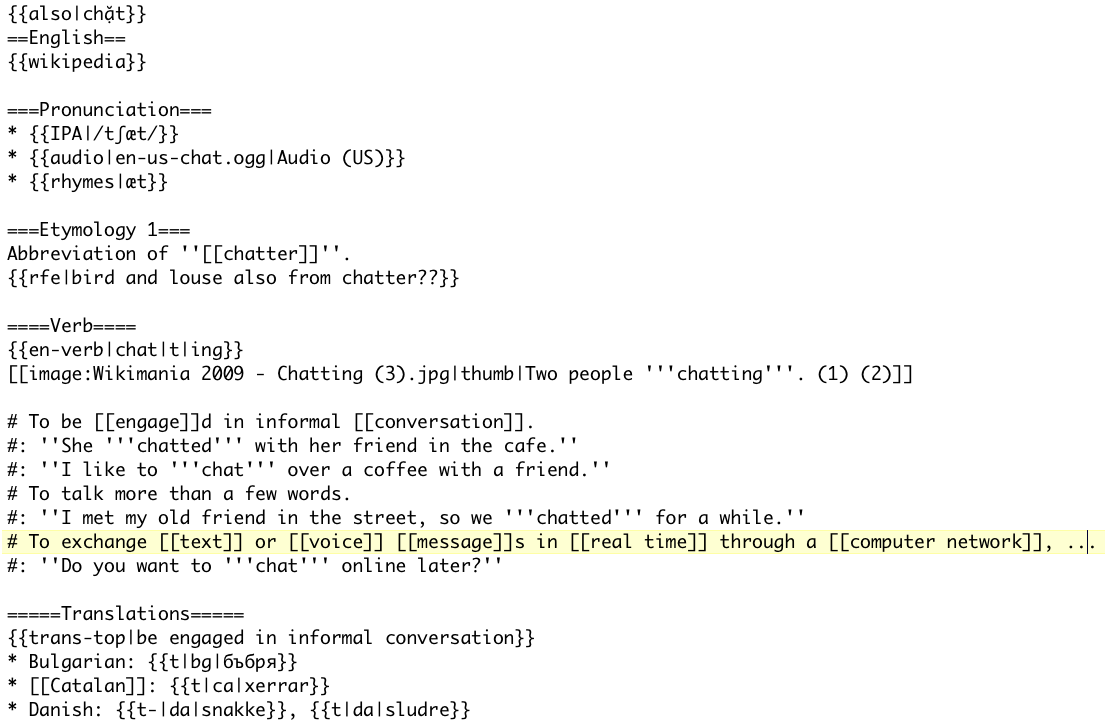
\includegraphics{chat1.png}
}
\caption{Excerpt of the entry chat in mediawiki syntax.}
\label{extr:sample}
\end{figure}

The dumps are extracted and encoded as UTF-16 text file. The extraction process goes through all pages in the dump file (using the provided xml based structure). Then each page is parsed using a finite state automaton implemented in java. The general abstract structure of entries is taken into account by a common abstract class while language specific details are refined through a language specific implementation class.

\section{Structuring Wiktionary Data as a WordNet}

\subsection{Specific Problems and Extraction Process}

Many project addressed wiktionary data extraction. \cite{sajous-EtAl-IceTAL2010} for instance provides an XML version of a 2010 wiktionary dump for French and English. \cite{ZeschMuellerGurevych2008} provide a free to use, but closed-source, java library to programmatically access the data of the English and German wiktionaries. Other projects did use wiktionary based data in NLP applications without providing details on the way this data was extracted.

However, few of them did address wiktionary server instances as a whole, interoperable lexical network. Moreover, we focus on building an open-source, reusable, efficient extractor and associated tools which will cope with wiktionary's constant evolution and proposes tools to avoid regression in successive data extractions. 

All the above mentioned project do stress that the data is sometimes erroneous and most of the time heterogeneous. For example, several entries will place the relations and translation after all part of speech sections. Moreover, different pages may use different conventions to identify parts of the entries. For instance, several templates may be used to identify the same section header as the encoding convention has evolved since the creation of a language wiktionary server. One can also find entries with syntactically incorrect template calls.

As stated in \cite{sajous-EtAl-IceTAL2010}, ``\emph{When merging information extracted from several languages, the homogenisation of the data structure often leads to the choice of the poorest one, resulting in a loss of information.}''. In this work we did not try to provide a uniform entry representation for all language but rather used a simple lexical network model to represent as much data as we can extract correctly from the wiktionary dumps. We also chose to ignore some of the structure to ease the extraction process. For instance, we do not keep information on etymology and we do not separate senses in homonym groups. Moreover, we do not try to attach relations to word senses, but we keep all sense annotations\footnote{e.g. many translations are grouped under an annotation that is usually a summary of a previous definition} in the network.

The extractor itself is structured as a general abstract class that contains all language independent processing and that is sub-classed by language specific processing. This way the addition of a new language mainly consists in identifying regular expressions that match the different elements structuring the entry (section headers) and the different element containing data to be extracted (translation templates, definition patterns, ...).

In these classes some heuristics are used to capture heterogeneous or erroneous data. But, as the wiktionary evolves (along with its conventions) and as the extraction program is adapted with new heuristics, one has to ensure that the extraction does not regress. For this, we use the Mulling tool provided by \cite{archer:2010} to compute the differences between extracted graphs. Such difference may be quickly evaluated and the extraction heuristics may be adopted or rejected based on this.

\subsection{Macro- and Micro- Structures}

Each language wiktionary is extracted as a lexical network. The English language network describes the English lemmas (giving their part of speech, definitions, lexical relations and translations) while the French one describes the French lemmas. However, all the lexical networks use the same node naming convention, based on language and canonical form, to denote the same lemma. For instance in any of the lexical networks, the node id \texttt{\#fra|chat} refers to the French form \emph{chat} while the id \texttt{\#eng|chat} refers to the English form. Interoperability is achieved through this convention and merging the lexical network files is enough to create a multilingual lexical resource.

This network contains 3 types of nodes: lemma nodes, definition nodes and Part of Speech nodes.

Nodes are related by several types of relations:

\begin{itemize}
\addtolength{\itemsep}{-0.5\baselineskip}
\item \texttt{pos} relation, which relates lemma and definition nodes to Part of Speech nodes,
\item \texttt{def} relation which relates a lemma node with its definitions,
\item \texttt{alt} relation which relates lemmas to their alternate spellings,
\item \texttt{ant} relation which relates lemmas to their antonyms,
\item \texttt{holo} relation which relates lemmas to their holonyms,
\item \texttt{hyper} relation which relates lemmas to their hypernyms,
\item \texttt{hypo} relation which relates lemmas to their hyponyms,
\item \texttt{mero} relation which relates lemmas to their meronyms,
\item \texttt{syn} relation which relates lemmas to their synonyms,
\item \texttt{trad} relation which related lemmas to their translation, this relation is annotated by the target language and by an optional glose that helps disambiguate the translated word sense.
\end{itemize}

In this very simple lexical network, all relation start from the lemma node and points to another lemma node. This is due to the fact there is o ways to identify the sense 
 
Using this very simple WordNet structure, we ignore many of the information available in wiktionaries, either because we do not want to use it in later processing or because it involves far more heuristics during data extraction.

%Figure \ref{chatWordNet} shows a sample of the extracted data in graphical format.

\section{Extracted Data}

\subsection{Size of the involved data}

At the time of writing, we extracted data from the most up to date dump files of English ($3.9$ Gb), French ($3.0$ Gb), German ($608$ Mb) and Portuguese ($390$ Mb) wiktionaries. The full extraction of the English wiktionary takes around 75 seconds on a 2.67 GHz Intel Xeon processor with enough memory to avoid swapping ($\sim 800$ Mb) as the lexical network is stored in memory during extraction.

Table \ref{extr:size} shows the size of the resulting networks.

%-rw-r--r--. 1 serasset geta 608M Oct 13 22:03 dewkt.xml
%-rw-r--r--. 1 serasset geta 3.9G Oct 13 22:02 enwkt.xml
%-rw-r--r--. 1 serasset geta 3.0G Oct 13 21:59 frwkt.xml
%-rw-r--r--. 1 serasset geta 390M Oct 13 22:03 ptwkt.xml

\begin{table}[htb]
\begin{minipage}{.9\linewidth}
\begin{tabular}{lrrrr}
\multicolumn{5}{l}{\textbf{Nodes in graphs}}\\
\hline
			& English & French & German & Portuguese\\
lemmas 	& $372773$  & $ 236215 $ & $51111$  & $35979$\\
definitions\footnote{The current English extraction script does not yet correctly recognize inflected forms. Hence, word nodes do not represent lemmas, but word forms and many word nodes are not related to a definition.}
			& $321637$ & 283493 & 72539 & 57281\\
other nodes\footnote{Other nodes are: lemmas that are not described in the wiktionary and lemmas or word forms in foreign languages}
			& 320994 & 315610 & 333549 & 186565\\
Total		& 1015404 & 835318 &457199 & 279825 \\
\multicolumn{5}{l}{\textbf{Relations in graphs}}\\
\hline
syn	& 59102& 53548& 74641&13228\\
qsyn	& 0& 2509 & 0&0\\
ant	& 9092& 8494& 34158&1650\\
holo	& 0  & 5491& 0 &0\\
mero	& 198& 4949&0 &0\\
hyper	& 906& 10438& 47785&2\\
hypo	& 2718& 16571& 53175&10\\
\end{tabular}
\end{minipage}
\caption{Size of the extracted lexical networks.}
\label{extr:size}
\end{table}

As can be seen in table \ref{extr:size} the number of relation is quite surprising in the German wiktionary. At the time of writing we do not have explanations on this figure and we still have to figure out if these relations are errors in the extraction process or problems in the wiktionary data itself. Errors are quite likely as the German wiktionary makes extensive use of nested macros which are difficult to correctly parse with our current automata based architecture.
%283493
%[serasset@brahms1 RAW_20111013]$ grep -c -- "-O- #def" en_extract.raw 
%321637
%[serasset@brahms1 RAW_20111013]$ grep -c -- "-O- #def" de_extract.raw 
%72539
%[serasset@brahms1 RAW_20111013]$ grep -c -- "-O- #def" pt_extract.raw 
%57281


%fr: 2176403 entries extracted in : 74163
%Semnet contains: 835318 nodes and 1372755 edges.
%
%de: 214984 entries extracted in : 90629
%Semnet contains: 457199 nodes and 742846 edges.
%
%en: 2803195 entries extracted in : 75379
%Semnet contains: 1015404 nodes and 1571179 edges.
%
%pt: 210889 entries extracted in : 13962
%Semnet contains: 279825 nodes and 386887 edges.
%
%[serasset@brahms2 RAW_20111013]$ grep -c -- "-O- #deu" de_extract.raw 
%51111
%[serasset@brahms2 RAW_20111013]$ grep -c -- "-O- #fra" fr_extract.raw 
%236215
%[serasset@brahms2 RAW_20111013]$ grep -c -- "-O- #eng" en_extract.raw 
%372773
%[serasset@brahms2 RAW_20111013]$ grep -c -- "-O- #por" pt_extract.raw 
%35979
%
%fr - alt : 39
%fr - ant : 8494
%fr - def : 323277
%fr - holo : 5491
%fr - hyper : 10438
%fr - hypo : 16571
%fr - mero : 4949
%fr - pos : 569820
%fr - qsyn : 2509
%fr - syn : 53548
%en - alt : 59
%en - ant : 9092
%en - def : 332743
%en - holo : 0
%en - hyper : 906
%en - hypo : 2718
%en - mero : 198
%en - pos : 732355
%en - qsyn : 0
%en - syn : 59102
%de - alt : 13
%de - ant : 34158
%de - def : 78849
%de - holo : 0
%de - hyper : 47785
%de - hypo : 53175
%de - mero : 0
%de - pos : 130875
%de - qsyn : 0
%de - syn : 74641
%pt - alt : 0
%pt - ant : 1650
%pt - def : 69547
%pt - holo : 0
%pt - hyper : 2
%pt - hypo : 10
%pt - mero : 0
%pt - pos : 107513
%pt - qsyn : 0
%pt - syn : 13228


%\subsection{Resulting lexical network}

\subsection{Example of extracted data}

Figure \ref{netsample} shows a excerpt of the extracted network for entry \texttt{\#eng|chat}.

\begin{figure}
\resizebox{.85\linewidth}{!}{%
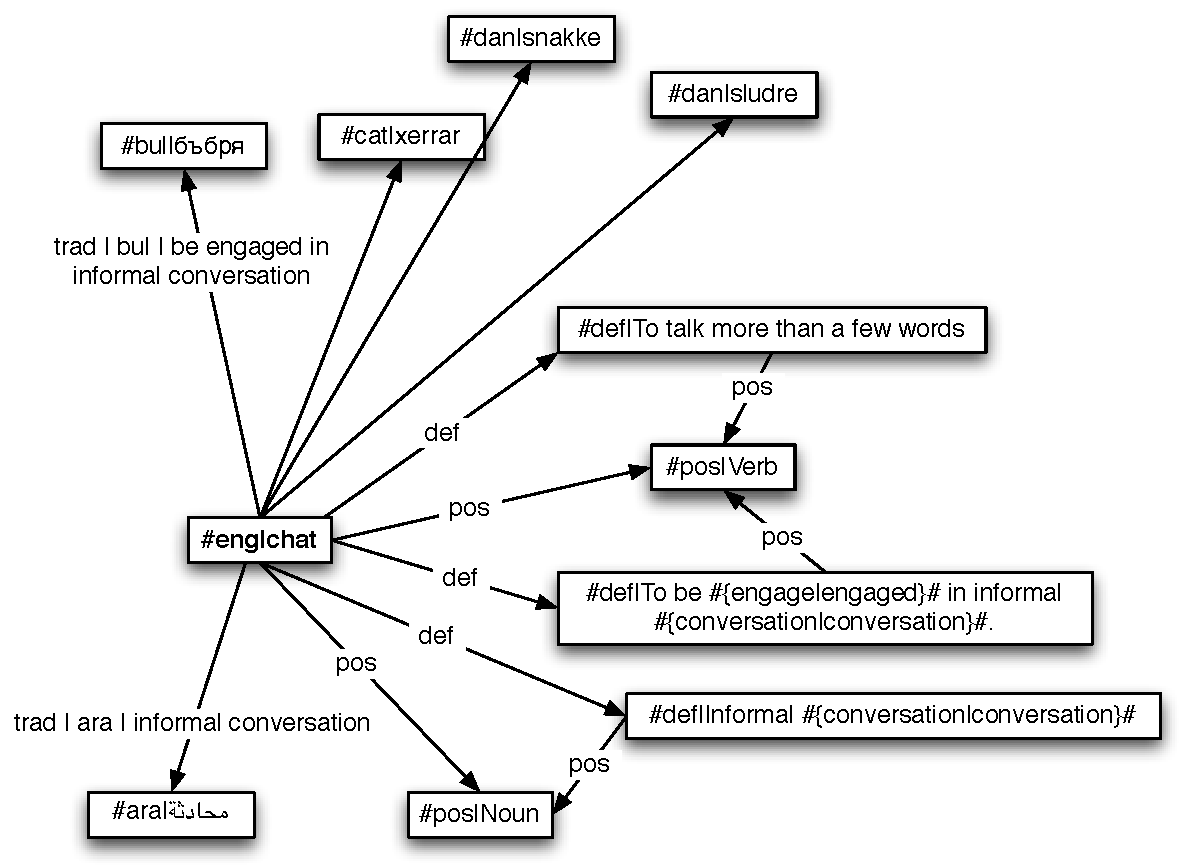
\includegraphics{chat.pdf}
}
\caption{Extract of the English \emph{chat} lexical network.}
\label{netsample}
\end{figure} 

\section{Conclusion}

Even if the current paper shows preliminary results, the main objective is to provide the extracted data as a lexical network formatted in RDF format so that the network is immediately usable by many existing tools (Ontology builders, Sparql query engines, reasoners...).

Our final objective is to create a tool that will be to wiktionary what dbpedia (\cite{Auer07dbpedia:a}] is to wikipedia. 

As a perspective, we will try to refine the lexical network structure to be compatible with the LMF standards (\cite{FRANCOPOULO:2006:INRIA-00121468:1}) to further improve interoperability of the extracted data with other resources or tools.



\bibliographystyle{apalike}      % basic style, author-year citations
\bibliography{biblio}   % name your BibTeX data base


\end{document}


Reference Information for Submission #387
Title:	 Wiktionary as a Multilingual Wordnet
Authors:	 Gilles Sérasset
Passcode:	 387X-H2G7G6F9P9
Confirmation Number:	387
File upload information
Abstract:	  (See Current Version)


%%%%%%%%%%%%%%%%%%%%%%%%%%%%%%% IGNORED
\section{Introduction}
\label{intro}
Les ressources lexicales contributives sont de plus en plus utilisées par les chercheurs en traitement automatique des langues comme source de données lexicales facilement accessibles. Parmi celles-ci figure le "wiktionary", pendant lexical de l'encyclopédie wikipédia, géré par la fondation \emph{wikimedia}. 

Les points forts du witkionnaire\footnote{\texttt{http://www.wiktionary.org}} (et des initiatives de la fondation \emph{wikimedia} en général) sont son caractère \emph{contributif} (de nombreuses personnes contribuent à hauteur de leur compétence à la construction de l'ensemble) et son caractère \emph{évolutif} (les données, en constante évolution, suivent l'usage de la langue). Ses points faibles sont son caractère \emph{contributif} (les contributeurs ne partagent pas de connaissance ni de méthodologie commune) et son caractère \emph{évolutif} (les choix de structures et de codages évoluent avec le temps, rendant obsolète des données autrefois abouties). Ce deux point faibles aboutissent à une assez forte incohérence interne des données disponible. 

Cet article propose une méthodologie d'extraction visant à construire un réseau lexical à partir des dumps de wiktionnaires de différentes langues. Cette méthodologie intègre une fonction d'évaluation de l'extraction \emph{relativement aux extractions précédentes} afin de valider les stratégies et heuristiques mises en place pour palier au manque de cohérence des données disponibles. 

Après avoir présenté brièvement la structure des données du wiktionnaire et celle des données qu'on en extrait, nous présenterons les outils utilisés pour rapidement mettre au point une méthodologie d'extraction intégrant une évaluation du processus d'extraction.

\section{Le Wiktionnaire}
\label{sec:wikt}

\subsection{Macro et micro structure}
\label{sec:wikt:struct}

réseau de divers serveurs. données multilingues sur chaque serveur. lien entre les serveurs, liens vers l'extérieur.

structure "simple" de dictionnaire papier.

\subsection{Format et taille des données}
\label{sec:wikt:form}

\subsection{Une incohérence inhérente à la ressource}
\label{sec:wikt:incoh}

Les incohérences proviennent de 2 phénomènes:

* La structure des articles est une structure visuelle, En ce sens, le wiktionnaire est un "machine readable dictionary" (cf nombreux travaux dans ce domaine...),

* Certaines entrées sont tout simplement mal codées (syntaxiquement incorrecte), mais la principale validation faite par les auteurs est "visuelle" et le langage wiki-wiki est très "tolérant aux fautes". 

* Certaines entrées ont été réalisées sans erreurs en utilisant des conventions qui ont pu évoluer depuis,

* Certaines informations n'ont pas été correctement structurées soit parce que la structure ne permettait pas de représenter correctement le phénomène, soit parce que le contributeur a fait une erreur,


\section{Le réseau lexical extrait}
\label{sec:lnet}

\subsection{Types de noeuds et relations}
\label{sec:lnet:onto}

\subsection{Exemple}
\label{sec:lnet:example}

\section{Méthodologie d'extraction}
\label{sec:metho}

\subsection{Vue générale}
\label{sec:metho:overview}

\subsection{Validation par non régression}
\label{sec:metho:valid}

\subsection{MulLing, un outil général de manipulation de graphes}
\label{sec:metho:mulling}

\section{Expérimentations}
\label{sec:expe}

\subsection{Un exemple d'heuristique et sa validation}
\label{sec:expe:heurist}

\subsection{État actuel de l'extracteur}
\label{sec:expe:currentState}

\section{Conclusion}
\label{sec:concl}

\section*{Remerciements}
\label{sec:thx}

%\paragraph{Paragraph headings} Use paragraph headings as needed.
\section*{Formating examples}
\begin{equation}
a^2+b^2=c^2
\end{equation}

% For one-column wide figures use
\begin{figure}
% Use the relevant command to insert your figure file.
% For example, with the graphicx package use
  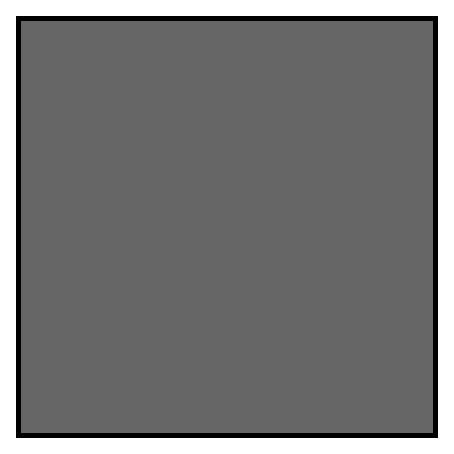
\includegraphics{example.eps}
% figure caption is below the figure
\caption{Please write your figure caption here}
\label{fig:1}       % Give a unique label
\end{figure}
%
% For two-column wide figures use
\begin{figure*}
% Use the relevant command to insert your figure file.
% For example, with the graphicx package use
  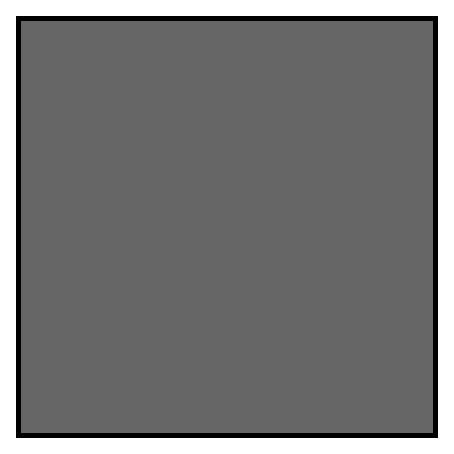
\includegraphics[width=0.75\textwidth]{example.eps}
% figure caption is below the figure
\caption{Please write your figure caption here}
\label{fig:2}       % Give a unique label
\end{figure*}
%
% For tables use
\begin{table}
% table caption is above the table
\caption{Please write your table caption here}
\label{tab:1}       % Give a unique label
% For LaTeX tables use
\begin{tabular}{lll}
\hline\noalign{\smallskip}
first & second & third  \\
\noalign{\smallskip}\hline\noalign{\smallskip}
number & number & number \\
number & number & number \\
\noalign{\smallskip}\hline
\end{tabular}
\end{table}


%\begin{acknowledgements}
%If you'd like to thank anyone, place your comments here
%and remove the percent signs.
%\end{acknowledgements}

% BibTeX users please use one of
\bibliographystyle{spbasic}      % basic style, author-year citations
%\bibliographystyle{spmpsci}      % mathematics and physical sciences
%\bibliographystyle{spphys}       % APS-like style for physics
\bibliography{biblio}   % name your BibTeX data base

% Non-BibTeX users please use
%\begin{thebibliography}{}
%
% and use \bibitem to create references. Consult the Instructions
% for authors for reference list style.
%
%\bibitem{RefJ}
% Format for Journal Reference
%Author, Article title, Journal, Volume, page numbers (year)
% Format for books
%\bibitem{RefB}
%Author, Book title, page numbers. Publisher, place (year)
% etc
%\end{thebibliography}

\end{document}
% end of file template.tex

